% The Potato Processor - Processor Datasheet
% (c) Kristian Klomsten Skordal 2015 <skordal@opencores.org>
% Report bugs and issues on <http://opencores.org/project,potato,bugtracker>

\documentclass[10pt,a4paper]{article}

\usepackage[pdftitle={The Potato Processor Datasheet},
	pdfauthor={Kristian Klomsten Skordal}]{hyperref}
\usepackage{graphicx}
\usepackage{multicol}
\usepackage{enumitem}
\usepackage{titlesec}
\usepackage{tabularx}
\usepackage[margin=2.0cm,includefoot,footskip=10pt]{geometry}
\usepackage[british]{babel}

\renewcommand{\familydefault}{\sfdefault}

\titleformat{\section}[block]{}{}{0pt}{\normalfont\large\bfseries}
\pagestyle{empty}

\setlength{\parindent}{0pt}
\setlist[itemize]{leftmargin=*,nosep}

\begin{document}

\begin{minipage}{0.5\textwidth}
\raggedright

\includegraphics[width=0.6\textwidth]{opencores.png}
\end{minipage}
\begin{minipage}{0.5\textwidth}
\raggedleft\Large\bf
\textsf{The Potato Processor\\Datasheet}
\end{minipage}

\vspace{0.5em}
\noindent\rule{\linewidth}{1pt}\\

\begin{minipage}[t]{0.48\textwidth}

\section{Architecture}
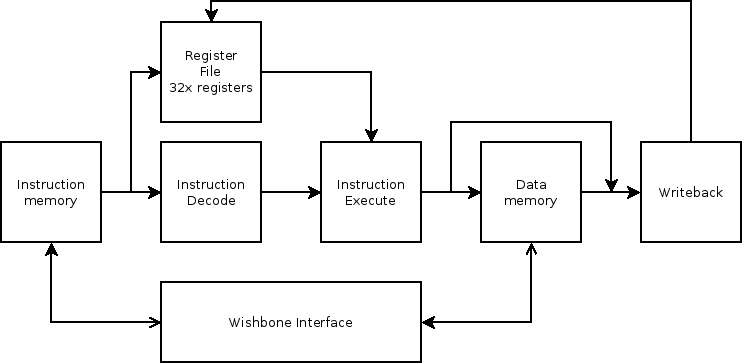
\includegraphics[width=\textwidth]{diagram.png}

\section{Features}

\begin{itemize}
\item Supports the complete 32-bit RISC-V base integer ISA (RV32I) version 2.0
\item Supports machine mode as defined by the RISC-V supervisor extensions version 1.7
\item Includes a hardware timer with microsecond resolution and compare interrupt
\item 8 IRQ inputs that can be invidually enabled
\item Classic 5-stage RISC pipeline
\item Instruction cache
\item Wishbone interface
\item Automatic test suite
\end{itemize}

\section{Interface}

The processor includes a wishbone interface conforming to the B4 revision of the
wishbone specification.\\

\begin{tabularx}{\textwidth}{|l|X|}
\hline
Interface type & Master \\
Address port width & 32 bits \\
Data port width & 32 bits \\
Data port granularity & 8 bits \\
Maximum operand size & 32 bits \\
Endianess & Little \\
Sequence of data transfer & In-order \\
\hline
\end{tabularx}

\section{Programming}

Tools for writing programmes for the RISC-V architecture are available from the
RISC-V project, at:\\[1em]
\url{https://github.com/riscv/riscv-tools}\\

Use the \texttt{new\_privileged\_isa} branch to get tools that work with the
current supervisor extensions.

\end{minipage}\hfill
\begin{minipage}[t]{0.48\textwidth}

\section{Application}
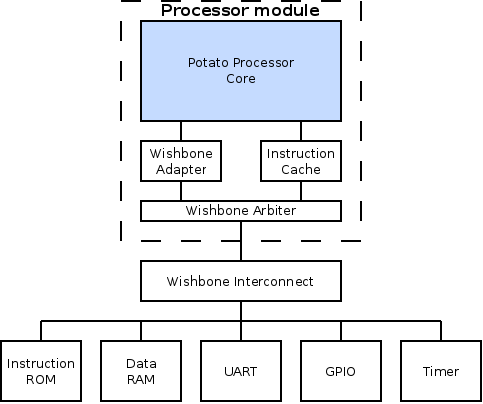
\includegraphics[width=\textwidth]{example.png}

\section{Signals}

The processor is provided by a VHDL module named \texttt{pp\_potato}. The signals of
the module are all active high and are as follows:\\

\begin{tabularx}{\textwidth}{|l|l|X|}
\hline
\textbf{Name} & \textbf{Width} & \textbf{Description} \\
\hline
\texttt{clk} & 1 & Processor clock \\
\texttt{timer\_clk} & 1 & 10~MHz timer clock \\
\texttt{reset} & 1 & Reset signal \\
\hline
\texttt{irq} & 8 & IRQ inputs \\
\hline
\texttt{wb\_adr\_out} & 32 & Wishbone address \\
\texttt{wb\_sel\_out} & 4 & Wishbone byte select \\
\texttt{wb\_cyc\_out} & 1 & Wishbone cycle \\
\texttt{wb\_stb\_out} & 1 & Wishbone strobe \\
\texttt{wb\_we\_out} & 1 & Wishbone write enable \\
\texttt{wb\_dat\_out} & 32 & Wishbone data output \\
\texttt{wb\_dat\_in} & 32 & Wishbone data input \\
\texttt{wb\_ack\_in} & 1 & Wishbone acknowledge \\
\hline
\end{tabularx}\\

Additional signals are used to implement a host-target interface used in the automatic testing
environment. These signals have names starting with \texttt{fromhost} and \texttt{tohost} and
should be left unconnected for normal use.\\

\section{Specifications}

The base RISC-V instruction set and the privileged extensions are available in the
specifications published at:\\

\url{http://riscv.org/download.html}.

\end{minipage}

\vfill
\noindent\rule{\linewidth}{1pt}
{\small
Project page: \url{http://opencores.org/project,potato}\\
Report bugs and issues on \url{http://opencores.org/project,potato,bugtracker}}

\end{document}


